\documentclass[11pt]{article}

\usepackage{array}
\usepackage{graphicx}

\newcolumntype{C}[1]{>{\centering\arraybackslash}m{#1}}

\begin{document}

\centering
\begin{tabular}{||C{6cm}|C{6cm}||}
\hline
\textbf{Bilder} & \textbf{Titel} \\ \hline
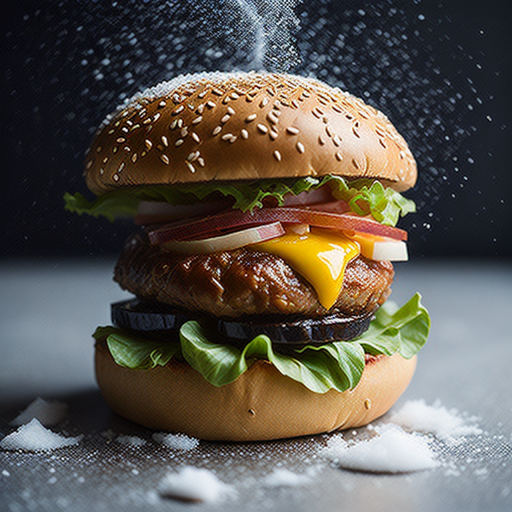
\includegraphics[width=0.7\linewidth]{Burger.png} & Burger \\
\hline
\rotatebox{90}{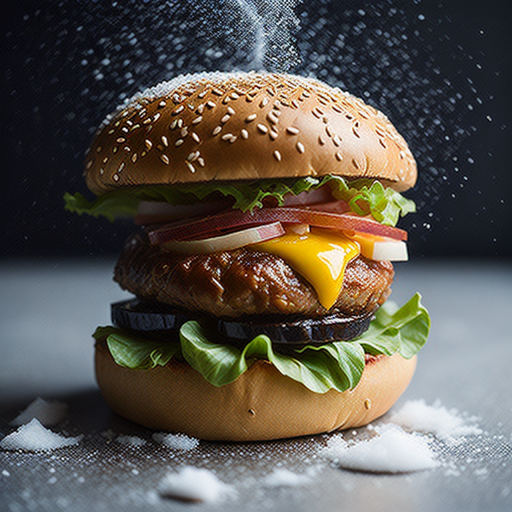
\includegraphics[width=0.4\linewidth]{Burger.png}} & \rotatebox{90}{{\fontsize{7pt}{9pt}\selectfont Rotated Burger}} \\
\hline

\includegraphics[width=0.7\linewidth]{Pizza.png} & Pizza \\
\hline
\rotatebox{180}{
\includegraphics[width=0.4\linewidth]{Pizza.png}} & \rotatebox{180}{{\fontsize{7pt}{9pt}\selectfont Upside down Pizza}} \\
\hline
\end{tabular}

\end{document}
